\documentclass{beamer}
\usepackage[utf8]{inputenc}
\usepackage{lmodern}
\usepackage[ngerman]{babel}
\usepackage{listings}
\usepackage{hyperref}
\usepackage{color}
\usepackage{todonotes}


\definecolor{darkred}{rgb}{0.75,0,0.3}
\usetheme{Ilmenau}
\usecolortheme{beaver}
\setbeamercovered{invisible}
\beamertemplatenavigationsymbolsempty % macht die Navigationsleiste weg
\setbeamercolor{block body}{bg=darkred!7.5}
\setbeamercolor{block title}{bg=darkred}
\setbeamercolor*{item}{fg=darkred!90}

\lstset{
  basicstyle=\footnotesize
}

\title{Ist die Disruption der Demokratie noch aufzuhalten?}
\subtitle{}
\author{Arne Struck \& Kim Möller}
\institute{Universität Hamburg, Fachschaft Informatik, Des Googles Kern}
\date{\today}

\begin{document}
\begin{frame}
\maketitle
\end{frame}

\begin{frame}{}
\tableofcontents
\end{frame}

\section{Grundlage des Datenschutzes}
\subsection{Datenschutzrichtlinien}
\begin{frame}{Die Entwicklung des Datenschutzes}
\begin{figure}[h]
\begin{center}
	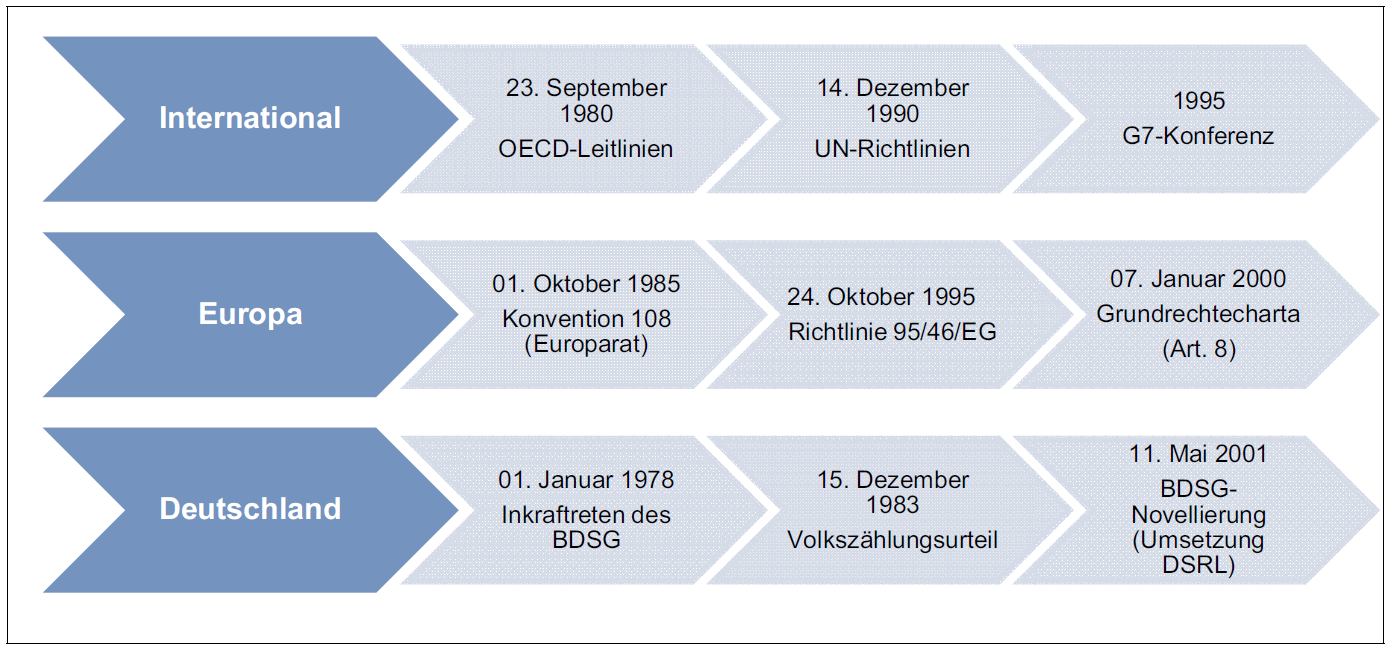
\includegraphics[scale=0.28]{pics/datenschutz.png}
\end{center}
\caption{Entwicklung des Datenschutzes (Quelle: \cite{europData})}
\label{pic:datenschutz}
\end{figure}
\end{frame}

\begin{frame}{Richtlinie 95/46/EG}
\begin{itemize}
	\item Richtlinie der Europäischen Gemeinschaft
	\item 1995 erlassen
	\item Schutz der Privatsphäre von natürlichen Personen bei der Verarbeitung von personenbezogenen Daten
	\item Drittstaatenregelung
\end{itemize}
\end{frame}



\begin{frame}{Weltweiter Stand des Datenschutzes}
\begin{figure}[h]
\begin{center}
	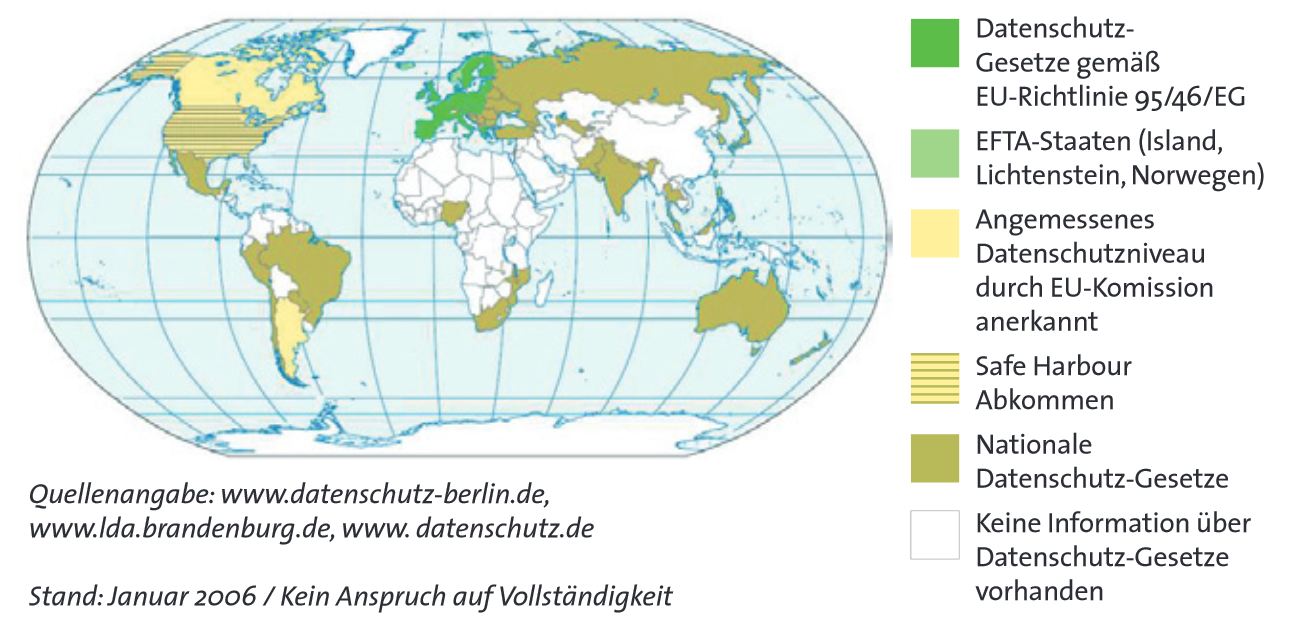
\includegraphics[scale=0.28]{pics/datenschutzstand.png}
\end{center}
\caption{Einschätzung des weltweiten Standes zum Thema Datenschutz}
\label{pic:worldmap}
\end{figure}
\end{frame}

\subsection{Safe harbor Abkommen}
\begin{frame}{Safe harbor Abkommen}
\underline{Safe harbor privacy principles}
\begin{itemize}
	\item Informationspflicht
	\item Wahlmöglichkeit
	\item Weitergabe
	\item Sicherheit
	\item Datenintegrität
	\item Auskunftsrecht
	\item Durchsetzung
\end{itemize}
\todo[inline]{sieht komisch aus, mit leerer rechten seite}
\end{frame}

\section{Chancen des Datenschutzes}
\begin{frame}{}
\todo[inline]{Placeholder}
\end{frame}


\subsection{Datenschutzgrundverordnung}
\begin{frame}{}
\todo[inline]{Placeholder}
\end{frame}

\section{Netzpolitik}
\subsection{Netzneutralität}
\begin{frame}{Netzneutralität}
\begin{block}{Definition}
	Gleichberechtigte Transport aller Daten in Datennetzen
\end{block}
\uncover<2>{
\quad \\
\underline{Status:}
\begin{itemize}
	\item Status in der EU: Parlament (meist) pro, Rat contra
	\item Status USA: Obama spricht für gesetzlich festgelegte Netzneutralität
	\item Status Deutschland: Regierung (durch Merkel) spricht sich gegen Netzneutralität aus
\end{itemize}
\todo[inline]{keine ahnung, ob gut so}
}
\end{frame}

\begin{frame}{Pro Contra}
\begin{columns}[t]
    \begin{column}{.5\textwidth}      	
      	\begin{block}{Pro}
		\begin{itemize}
			\item wichtig für Veränderung \(\Rightarrow\) Konkurrenz für Monopole
			\item \todo[inline]{Zu ende führen}
		\end{itemize}
		\end{block}
    \end{column}
	\begin{column}{.5\textwidth}
		\uncover<2> {
		\begin{block}{Contra}
       	\begin{itemize}
			\item Netzneutralität tötet
			\item \todo[inline]{Zu ende führen}
       	\end{itemize}
		\end{block}
		}
	\end{column}
\end{columns}
\end{frame}

\begin{frame}{Die Spitzenpolitik zu Netzneutralität}
\begin{center}
\href{https://www.youtube.com/watch?v=_ZaaSC7Eg4s}{
	\centering
	
\includegraphics[scale=0.15]{pics/Play-button.png}
}
\end{center}
\end{frame}



\section{Konzerne übernehmen das Internet}
\subsection{Internet.org}
\begin{frame}{Was ist Internet.org}
\begin{itemize}
	\item Non Profit Organisation
	\item Kooperation mehrerer namhafter Unternehmen, initiiert von Facebook
	\item Ziele: 
	\begin{itemize}%[<+->]
		\item kostenloses (Grund-)Internet für die Welt
		\item Effiziente Lösung
		\item Kooperation als Geschäftsmodell
	\end{itemize}
\end{itemize}
\end{frame}

\begin{frame}{Probleme}
\begin{itemize}
	\item Kein echter Internetzugang, da nur von Facebook akzeptierte Dienstleistungen zugelassen (bspw: zero rating Klausel)
	\item erhobene Nutzungsdaten gehören Facebook
	\item einseitige nachträgliche Vertragsänderungen seitens Facebook möglich
	\item alle ''inkompatiblen'' Seiten nicht über Internet.org erreichbar
	\item in Drittweltländern mögliche Konkurrenz zu Grundbedürfnissen (finanziell)
	\item unsicher (bspw. kein TLS/SSL/HTTPS)
\end{itemize}
\end{frame}

\begin{frame}{Rezeption des Internets}
\begin{figure}[h]
\begin{center}
	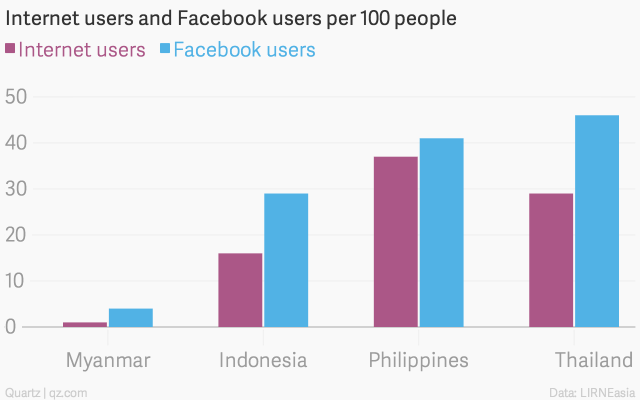
\includegraphics[scale=0.35]{pics/internetvsfacebook.png}
\end{center}
\caption{\begin{footnotesize}
Internet- und Facebooknutzer in Prozent der Bevölkerung (Quelle: \cite{quartz:inetvfb})
\end{footnotesize}
}
\label{pic:inetvfb}
\end{figure}
\end{frame}

\section*{Quellen}
\setbeamertemplate{bibliography item}{\insertbiblabel}
\setbeamercolor{bibliography item}{parent=palette primary}
\setbeamercolor*{bibliography entry title}{parent=palette primary}
\begin{frame}[shrink=10]{Quellen}
\bibliographystyle{alpha}
\bibliography{literature}
\todo[inline]{nur Bild- oder auch Infoquellen?}
\end{frame}

\end{document}
